\documentclass[11pt,largemargins]{homework}
\usepackage{xeCJK}
\usepackage{amsthm}
\usepackage{amsmath}

\usepackage{tikz}
\usetikzlibrary{calc}
\usepackage{amsmath,amssymb}
\usepackage{tikz-cd}
\usetikzlibrary{fit}
\usetikzlibrary{arrows.meta}
\usepackage{enumitem}


\newcommand{\hwname}{蘇則宇}
\newcommand{\hwemail}{B11201005}
\newcommand{\hwtype}{Homework}
\newcommand{\hwnum}{10}
\newcommand{\hwclass}{Modern Algebra I}
\newcommand{\hwlecture}{}
\newcommand{\hwsection}{}

% This is just used to generate filler content. You don't need it in an actual
% homework!
\usepackage{lipsum}
\begin{document}
	\maketitle
	\question
	\begin{enumerate}[label=(\alph*)]
		\item 
		Consider the following commuting diagram:
		
		\begin{center}
		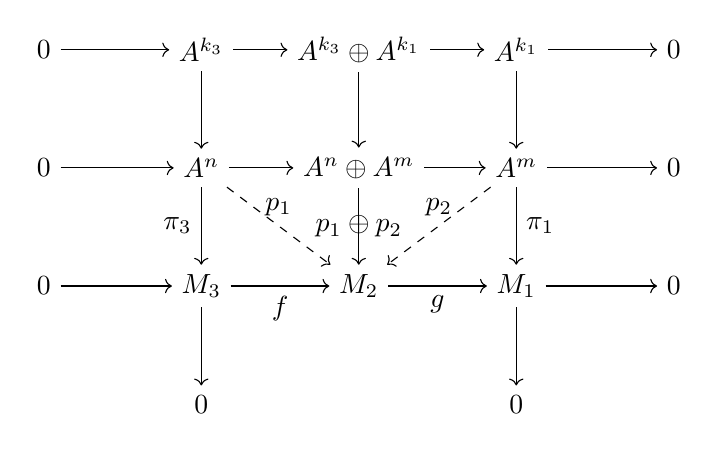
\begin{tikzpicture}
			\node (ol) at (0,0) {$0$};
			\node (An) at (2,0) {$A^n$};
			\node (Anm) at (4,0) {$A^n\oplus A^m$};
			\node (Am) at (6,0) {$A^m$};
			\node (or) at (8,0) {$0$};
			
			\draw[->] (ol) to (An);
			\draw[->] (An) to (Anm);
			\draw[->] (Anm) to (Am);
			\draw[->] (Am) to (or);
			
			\node (oll) at (0,-1.5) {$0$};
			\node (M3) at (2,-1.5) {$M_3$};
			\node (M2) at (4,-1.5) {$M_2$};
			\node (M1) at (6,-1.5) {$M_1$};
			\node (orr) at (8,-1.5) {$0$};
			
			\draw[->] (oll) to (M3);
			\draw[->] (M3) -- (M2) node[midway,below]{$f$};
			\draw[->] (M2) -- (M1) node[midway,below]{$g$};
			\draw[->] (M1) to (orr);
			
			\node (olll) at (0,1.5) {$0$};
			\node (K3) at (2,1.5) {$A^{k_3}$};
			\node (K2) at (4,1.5) {$A^{k_3}\oplus A^{k_1}$};
			\node (K1) at (6,1.5) {$A^{k_1}$};
			\node (orrr) at (8,1.5) {$0$};
		
			
			\draw[->] (olll) to (K3);
			\draw[->] (K3) to (K2);
			\draw[->] (K2) to (K1);
			\draw[->] (K1) to (orrr);
			
			\draw[->] (K3) to (An);
			\draw[->] (An) -- (M3) node[midway,left]{$\pi_3$};
			\draw[->] (K2) to (Anm);
			\draw[->] (Anm)--(M2) node[midway]{$p_1\oplus p_2$};
			\draw[->] (K1) to (Am);
			\draw[->] (Am) -- (M1) node[midway,right]{$\pi_1$};
			
			\node (odl) at (2,-3) {$0$};
			
			\node (odr) at (6,-3) {$0$};
			
			\draw[->] (M3) to (odl);
		
			\draw[->] (M1) to (odr);
			
			\draw[->,dashed] (An)--(M2) node[midway,above]{$p_1$};
			\draw[->,dashed] (Am)--(M2) node[midway,above]{$p_2$};
		\end{tikzpicture}
		\end{center}
		Where $p_1$ is defined to be $f\circ \pi_3$, and since $A^m$ is free (hence projective), exists $p_2:A^m\rightarrow M_2$ s.t. $g\circ p_2=\pi_1$.\\
		Now it remains to show $p_1\oplus p_2$ is surjective.\\
		By five lemma, $p_1\oplus p_2$ is surjective, hence $M_2$ can be generated by $n+m$ elements, and the kernel of $p_1\oplus p_2$ is an image of $A^{k_3}\oplus A^{k_1}$, which is also finitely generated. So $M_2$ is finitely presented. 
		\item 
		Let $A^k\xrightarrow{\phi} A^m\xrightarrow{\pi} M_2\rightarrow 0$ and $A^n\rightarrow M_3\rightarrow 0$, and $M_3\xrightarrow{f}M_2\xrightarrow{g}M_1$\\
		Since $g\circ \pi:A^m\rightarrow M_1$ is surjective, $M_1$ is finitely generated. Consider $K=\text{ker}(g\circ\pi)=\pi^{-1}(M_3)$ (view $M_3$ as a submodule of $M_2$).\\
		Let $x\in K$, then $\pi(x)\in M_3$, so is a finite sum $\pi(x)=\sum_{i=1}^{n} a_i v_i$.\\
		Choose $y_i\in A^m$ s.t. $\pi(y_i)=v_i$, then $x-\sum_{i=1}^{n}a_iy_i\in \text{ker}(\pi)=\text{im}(\phi)$, which is finitely generated. Let $z_1,...,z_k\in A^{m}$ generates $\text{ker}(\pi)$, then $\lbrace z_1,...,z_k,y_1,...,y_n \rbrace$ generates $K$. Hence $M_1$ is finitely presented.
		\end{enumerate}
	\question
	\begin{enumerate}[label=(\alph*)]
		\item Let $G\neq 0$ and $n=|G|<\infty$ be the order of $G$, choose $a\neq 0$, then no $g\in G$ satisfies $n\cdot g=a$. 
		\item Let $F_X$ be free over $X$, and choose a fixed $x\in X$. $F_{\lbrace x \rbrace}\cong \mathbb{Z}$ is a subgroup of $F_X$, let $1_x$ be the generator.\\
		Assume $F_X$ is divisible, and let $n=2$, then there is some $g=\sum_{i=1}^{n}a_{i}1_{x_i}$ , $a_i\in\mathbb{Z},$ s.t. $2g=1_x$.\\
		Define a mapping:
		\begin{align*}
			X&\xrightarrow{\phi} \mathbb{Z}\\
			a&\mapsto \begin{cases}
				1 \text{ if } a=x,\\
				0 \text{ otherwise.}
				\end{cases}
		\end{align*}
		, then there is an unique extension $\tilde{\phi}:F_X\rightarrow \mathbb{Z}$, and $\tilde{\phi}(2g)=\tilde{\phi}(1_x)=1$.\\
		Therefore $x_j=x$ for some $j$ and $2\cdot a_j=1 $, but this is impossible in $\mathbb{Z}$, so $F_X$ is not divisible.
		\item Let $D$ be divisible, and consider quotient group $D/K$.\\
		For $x+K\in D/K$ and $n\in\mathbb{N}-\lbrace 0 \rbrace$, there exists some $d\in D$ s.t. $n\cdot d=x$, hence $n\cdot (d+K)=n\cdot d+K=x+K$.
	\end{enumerate}
	\question
	$\mathbb{Z}$ is a free $\mathbb{Z}-$mod, hence is projective.\\
	To prove $\mathbb{Z}$ is not injective, consider the following diagram:\begin{center}
			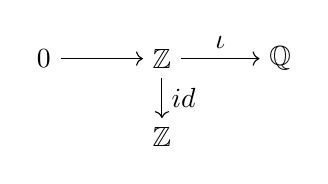
\begin{tikzpicture}
				\node (o) at (0,0) {$0$};
				\node (Z1) at (1.5,0) {$\mathbb{Z}$};
				\node (Q) at (3,0) {$\mathbb{Q}$};
				\node (Z2) at (1.5,-1) {$\mathbb{Z}$};
				
				\draw[->] (o)--(Z1);
				\draw[->] (Z1)--(Q) node[midway,above]{$\iota$};
				\draw[->] (Z1)--(Z2) node[midway,right]{$id$};
			\end{tikzpicture}
	\end{center}
	If $\mathbb{Z}$ is injective, then there is some $f:\mathbb{Q}\rightarrow\mathbb{Z}$ making the diagram commute. Clearly $f(z)=z$ for integer $z$, and suppose $f(\frac{1}{2})=z_1\in\mathbb{Z}$, then $2f(\frac{1}{2})=1=2z_1$, which is impossible. So $\mathbb{Z}$ is not injective.\\
	Since $\mathbb{Q}$ is divisible, hence is injective.\\
	Since $\mathbb{Z}$ is a PID, every submodule of a free module is also free, suppose $\mathbb{Q}$ is projective, then it is a direct summand of some free $\mathbb{Z}-$mod, hence a $\mathbb{Z}-$submod of free module, hence is free.\\
	Since a $\mathbb{Z}-$mod homomorphism $\mathbb{Q}\rightarrow\mathbb{Z}$ is uniquely determined by the image of a single non-zero element, so $\mathbb{Q}$ can only be free of rank 1.($\mathbb{Z}$ is PID, so rank is well-defined), but then $\mathbb{Q}\cong\mathbb{Z}$, a contradiction.
	\question
	Need to show for any short exact sequence of $B-$mod: 
	\begin{equation*}
		0\rightarrow N_3\rightarrow N_2\rightarrow N_1\rightarrow 0
	\end{equation*}
	, the sequence:
	\begin{equation*}
		0\rightarrow N_3\otimes_B (B\otimes_A M)\rightarrow N_2\otimes_B (B\otimes_A M)\rightarrow N_1\otimes_B (B\otimes_A M)\rightarrow 0
	\end{equation*}
	is also exact.\\
	Since tensor product is associative:
	\begin{equation*}
	N_i\otimes_B(B\otimes_A M)=(N_i\otimes_B B)\otimes_A M\\=N_i\otimes_A M
	\end{equation*}
	We have the following diagram:
	\begin{center}
	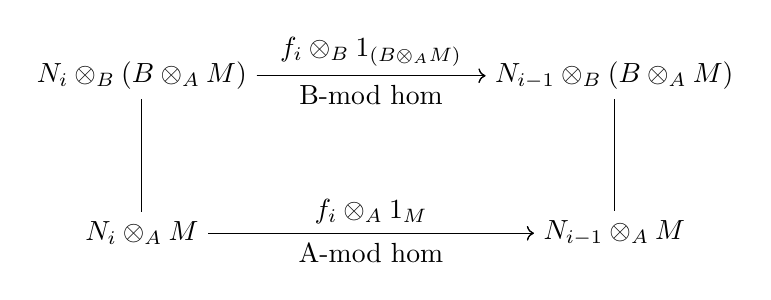
\begin{tikzpicture}
		\node(BL) at (0,0) {$N_i\otimes_B(B\otimes_A M)$};
		\node(BR) at (6,0) {$N_{i-1}\otimes_B(B\otimes_A M)$};
		\node(AL) at (0,-2) {$N_i\otimes_A M$};
		\node(AR) at (6,-2) {$N_{i-1}\otimes_A M$};
		
		\draw[->] (BL)--(BR) node[midway,above]{$f_i\otimes_B 1_{(B\otimes_A M)}$};
		\draw[->] (BL)--(BR) node[midway,below]{B-mod hom};
		\draw[->] (AL)--(AR) node[midway,above]{$f_i\otimes_A 1_{M}$};
		\draw[->] (AL)--(AR) node[midway,below]{A-mod hom};
		\draw[-] (BL) to (AL);
		\draw[-] (BR) to (AR);
	\end{tikzpicture}
	\end{center}
	Since $M$ is a flat $A-$mod, the following diagram commute:
	\begin{equation*}
		0\rightarrow N_{3}\otimes_A M \rightarrow N_{2}\otimes_A M\rightarrow N_{1}\otimes_A M\rightarrow 0
	\end{equation*}
	So Im$(f_i\otimes_A 1_M)=$Ker$(f_{i-1}\otimes_A 1_M)$, hence Im$(f_i\otimes_B 1_{(B\otimes_A M)})=$Ker$(f_{i-1}\otimes_B 1_{(B\otimes_A M)})$, hence the functor $\bullet \otimes_B M_B$ is exact.
\end{document}